\documentclass{beamer}
 
\usepackage[utf8]{inputenc}
\usepackage{svg}
\usepackage{tikz}
\usepackage{amsmath}
\usepackage[customcolors]{hf-tikz}
\usepackage[round]{natbib}

\usepackage{hyperref}
\usepackage{cleveref}
\usepackage[english]{babel}
\usepackage{graphicx}

% animate slides
\usepackage{animate}

% strikeout
\usepackage{ulem}

% appedix
\usepackage{appendixnumberbeamer}

% colors
\definecolor{amber}{rgb}{1.0, 0.75, 0.0}
\definecolor{generator}{rgb}{0.67, 0.9, 0.93}
\definecolor{discriminator}{rgb}{0.89, 0.44, 0.48}
\definecolor{generated}{rgb}{0.82, 0.1, 0.26}
\definecolor{real}{rgb}{0.0, 0.5, 0.0}
\definecolor{goldenyellow}{rgb}{1.0, 0.87, 0.0}

% quotation
\usepackage{ifxetex,ifluatex}
\usepackage{etoolbox}
\usepackage{xcolor}

\usepackage{tikz}

\usepackage{framed}

% conditional for xetex or luatex
\newif\ifxetexorluatex
\ifxetex
\xetexorluatextrue
\else
\ifluatex
\xetexorluatextrue
\else
\xetexorluatexfalse
\fi
\fi
%
\ifxetexorluatex%
\usepackage{fontspec}
\usepackage{libertine} % or use \setmainfont to choose any font on your system
\newfontfamily\quotefont[Ligatures=TeX]{Linux Libertine O} % selects Libertine as the quote font
\else
\usepackage[utf8]{inputenc}
\usepackage[T1]{fontenc}
\usepackage{libertine} % or any other font package
\newcommand*\quotefont{\fontfamily{LinuxLibertineT-LF}} % selects Libertine as the quote font
\fi

\newcommand*\quotesize{60} % if quote size changes, need a way to make shifts relative
% Make commands for the quotes
\newcommand*{\openquote}
{\tikz[remember picture,overlay,xshift=-4ex,yshift=-2.5ex]
	\node (OQ) {\quotefont\fontsize{\quotesize}{\quotesize}\selectfont``};\kern0pt}

\newcommand*{\closequote}[1]
{\tikz[remember picture,overlay,xshift=1ex,yshift={#1}]
	\node (CQ) {\quotefont\fontsize{\quotesize}{\quotesize}\selectfont''};}

% select a colour for the shading
\colorlet{shadecolor}{amber!40!white}

\newcommand*\shadedauthorformat{\emph} % define format for the author argument

% Now a command to allow left, right and centre alignment of the author
\newcommand*\authoralign[1]{%
	\if#1l
	\def\authorfill{}\def\quotefill{\hfill}
	\else
	\if#1r
	\def\authorfill{\hfill}\def\quotefill{}
	\else
	\if#1c
	\gdef\authorfill{\hfill}\def\quotefill{\hfill}
	\else\typeout{Invalid option}
	\fi
	\fi
	\fi}
% wrap everything in its own environment which takes one argument (author) and one optional argument
% specifying the alignment [l, r or c]
%
\newenvironment{shadequote}[2][l]%
{\authoralign{#1}
	\ifblank{#2}
	{\def\shadequoteauthor{}\def\yshift{-2ex}\def\quotefill{\hfill}}
	{\def\shadequoteauthor{\par\authorfill\shadedauthorformat{#2}}\def\yshift{2ex}}
	\begin{snugshade}\begin{quote}\openquote}
		{\shadequoteauthor\quotefill\closequote{\yshift}\end{quote}\end{snugshade}}


\usetheme{metropolis}
 
 
\title[GAN]
{GAN - Theory and Applications}
  
\author
{Emanuele Ghelfi  \and \\ Paolo Galeone \and \\ Federico Di Mattia \and \\ Michele De Simoni \and \\ \href{https://github.com/zurutech/gans-from-theory-to-production}{github.com/zurutech/gans-from-theory-to-production}}
 

 
\titlegraphic{
	 \begin{picture}(0,0)
	\put(70,40){\makebox(0,0)[rt]{
	
\includegraphics[width=0.3\textwidth]{images/zuru.png}}}
\end{picture}
}
 
 
 
\begin{document}
 
{
  \usebackgroundtemplate{
  	\tikz[overlay,remember picture]
  	\node[opacity=.4, at=(current page.center)] {
  		\includesvg[width=0.5\textwidth]{images/pycon_x_logo.svg}};}
  \begin{frame}
    \titlepage
  \end{frame}
}


{
	\setbeamercolor{background canvas}{bg=black}
\begin{frame}[plain]
\centering
	\animategraphics[loop,autoplay,height=1\paperheight]{0.5}{images/stylegan/0990}{00}{10}
\end{frame}
}

\begin{frame}{Overview}
\setbeamertemplate{section in toc}[sections numbered]
\tableofcontents[hideallsubsections]
\end{frame}


\section{Introduction}

\begin{frame}
	 \begin{shadequote}[c]{Yann LeCun, Director, Facebook AI}
		\Large Generative Adversarial Networks is the \textbf{most interesting idea in the last ten years} in machine learning.
	\end{shadequote}
\vspace{-0.5cm}
\begin{figure}
	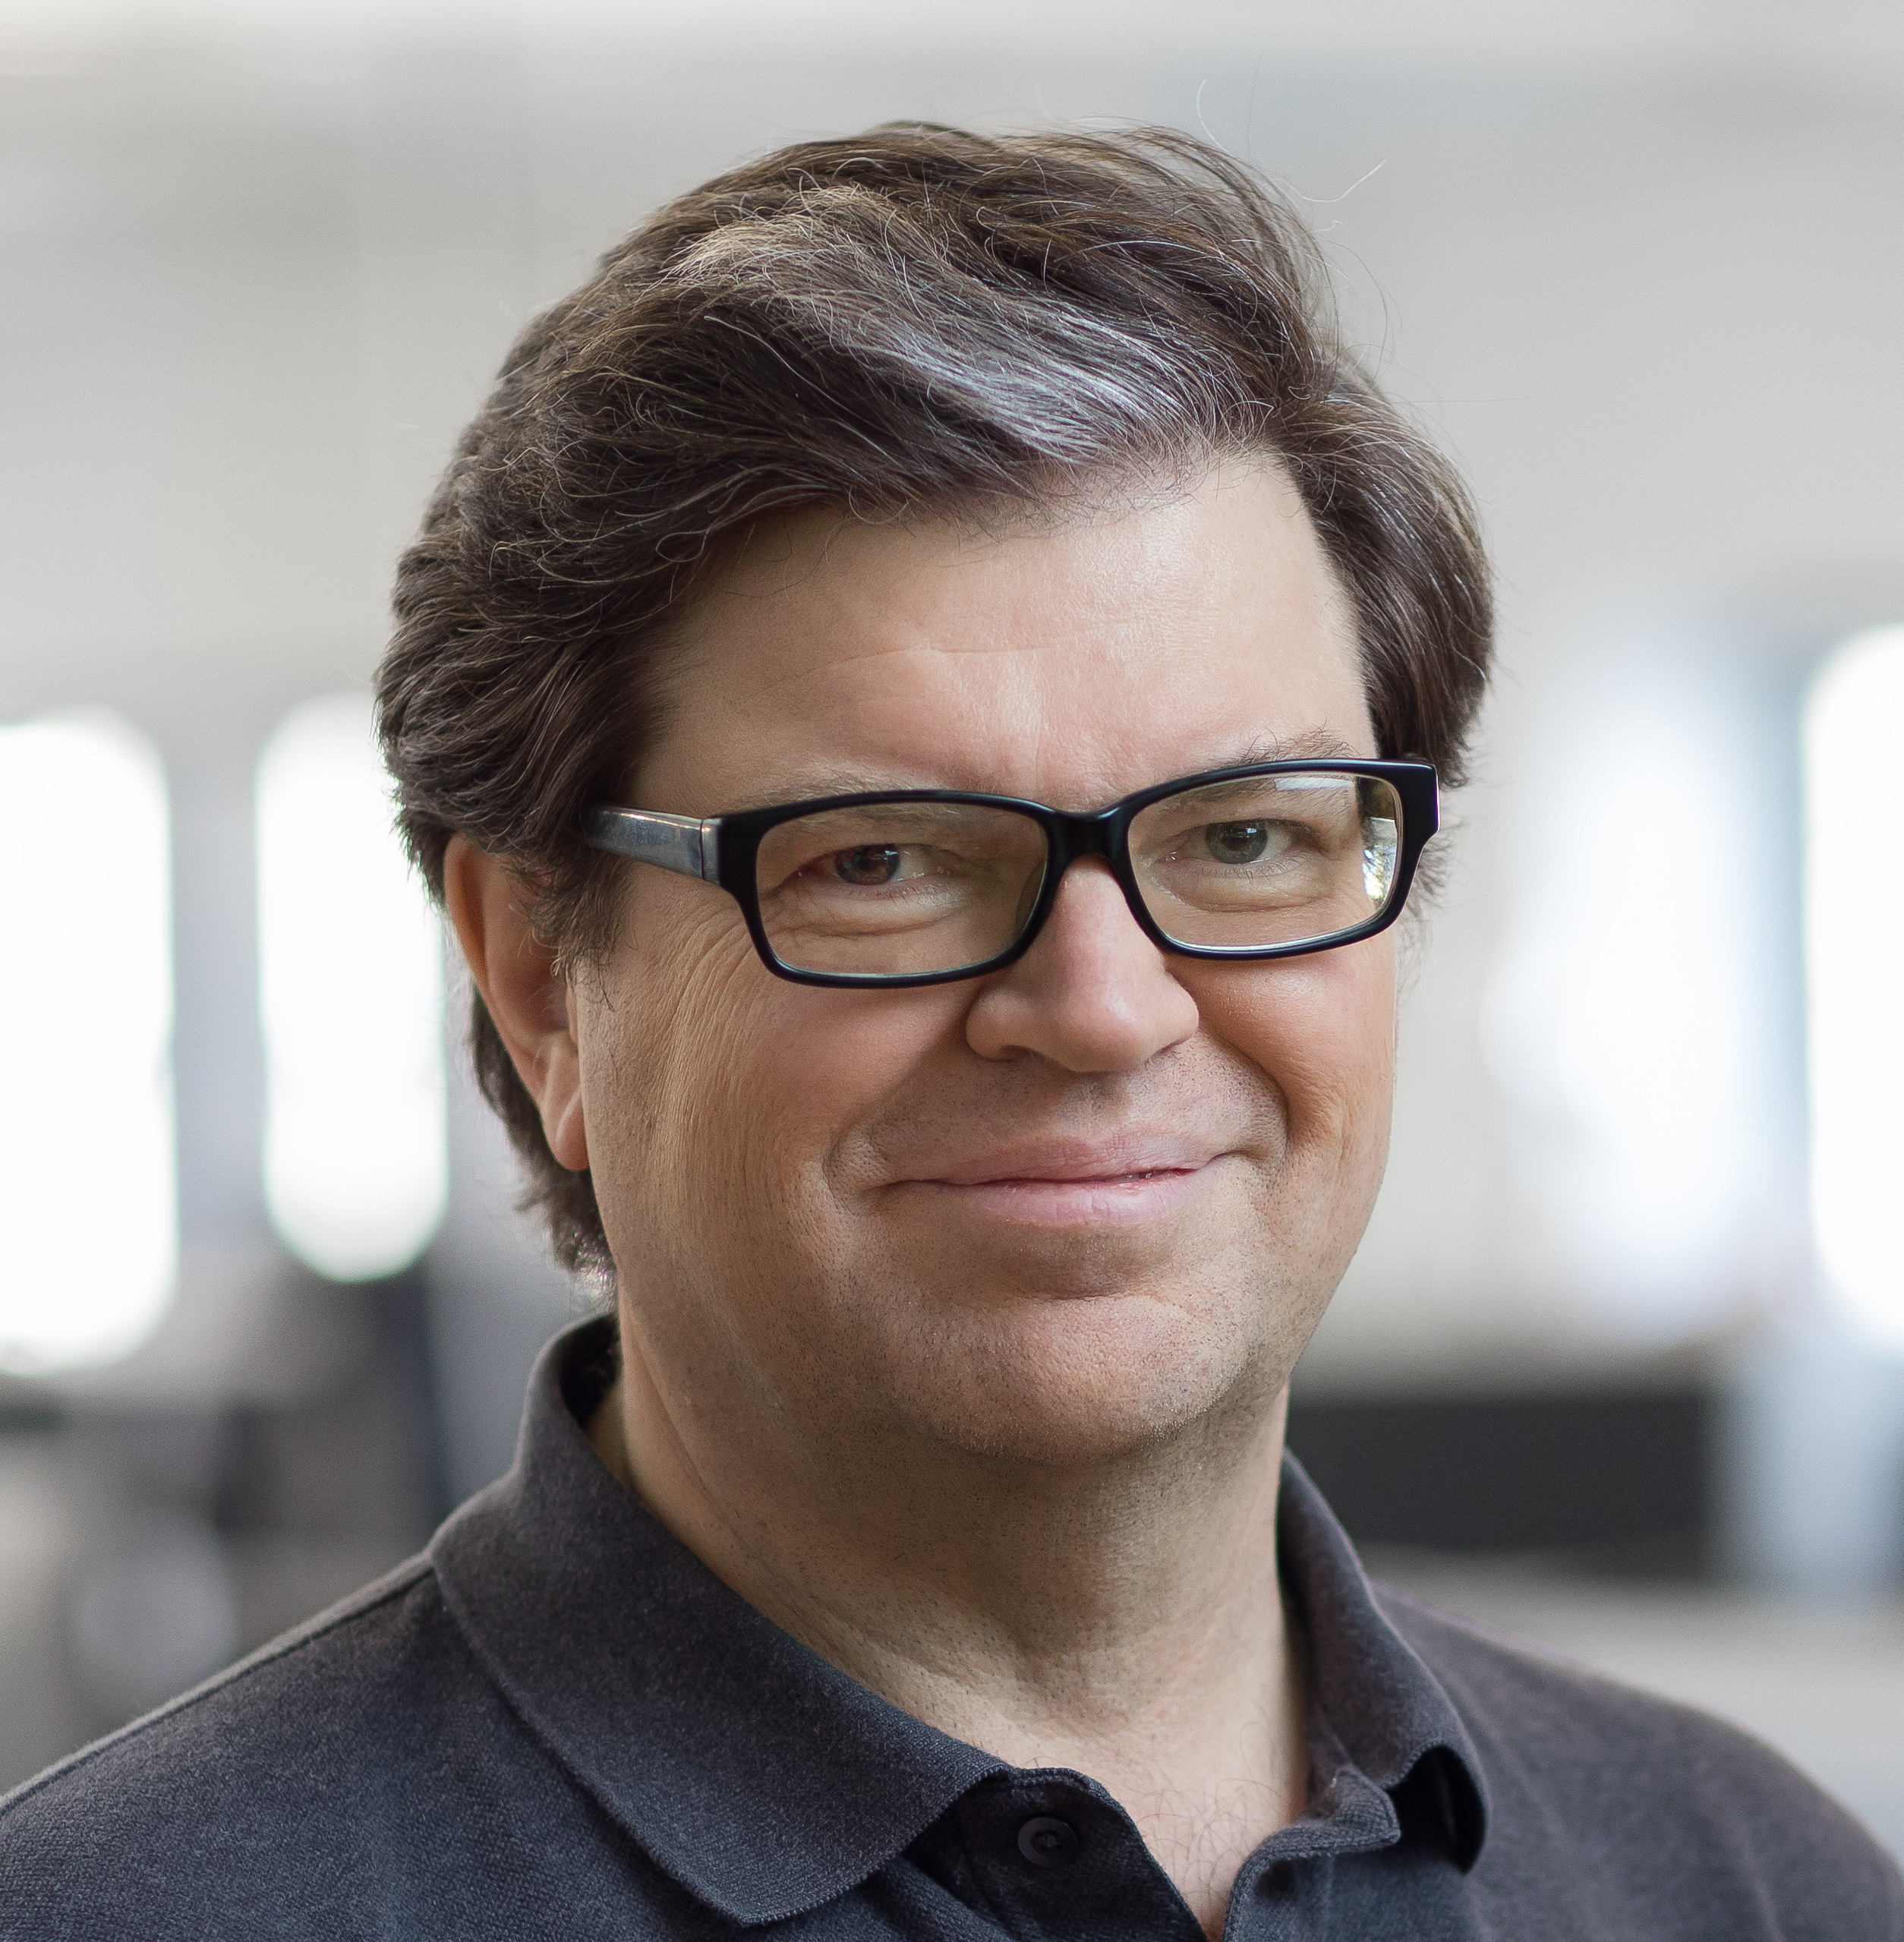
\includegraphics[width=0.7\paperheight]{images/lecun3.jpg}
\end{figure}
\end{frame}

\begin{frame}
	\frametitle{Generative Adversarial Networks}
	
	Two components, the \textbf{generator} and the \textbf{discriminator}:
	\begin{itemize}
			\item The \textbf{generator} G needs to capture the data distribution.
			\item The \textbf{discriminator} D estimates the probability that a sample comes from the training data rather than from G.
	\end{itemize}
	
	\begin{figure}
		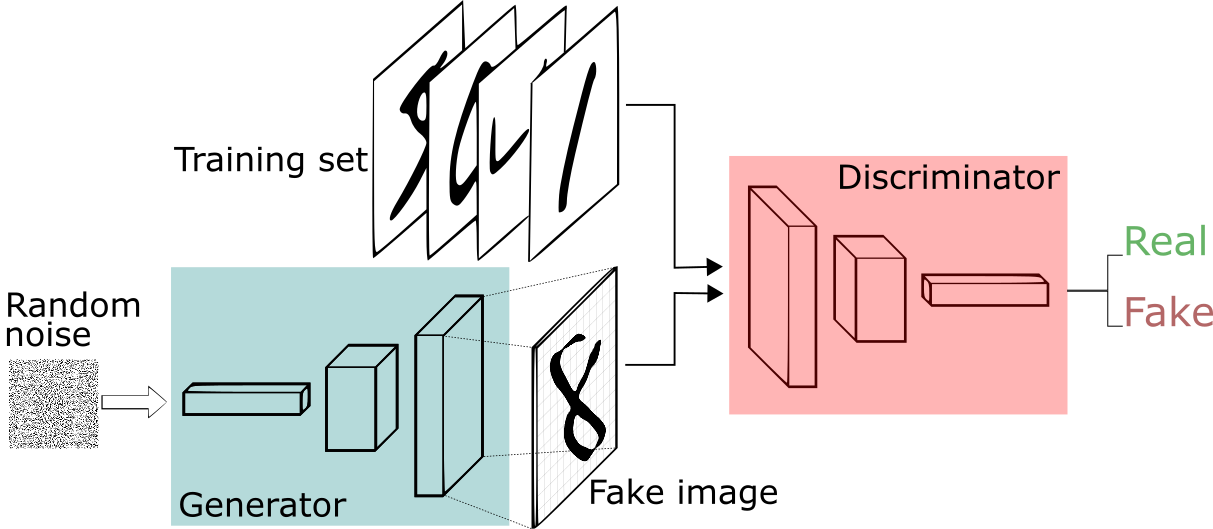
\includegraphics[width=0.9\textwidth]{images/GANs.png}
		\caption{Credits: \cite{silvaIntuitiveIntroductionGenerative2018} }
	\end{figure}

\end{frame}

\begin{frame}
	\frametitle{Generative Adversarial Networks}
	GANs game:
	\only<1>{
		\begin{equation*}
		 \min_G \max_D V_{GAN}(D,G) = \underset{x \sim p_{data}(x)}{\mathbb{E}} [\log D(x)]  +\underset{z \sim p_z(z)}{\mathbb{E}}[\log(1 - D(G(z)))]
		\end{equation*}
	}
	
	\only<2>{
			\begin{equation*}
			\min_G \max_D V_{GAN}(D,G) =\color{real}\underbrace{ \color{black} \underset{x \sim p_{data}(x)}{\mathbb{E}} [\log D(x)]}_{\text{real samples}} \color{black}  +\underset{z \sim p_z(z)}{\mathbb{E}}[\log(1 - D(G(z)))]
			\end{equation*}
	}
	
	\only<3>{
			\begin{equation*}
			\min_G \max_D V_{GAN}(D,G) = \color{real} \underbrace{\color{black} \underset{x \sim p_{data}(x)}{\mathbb{E}} [\log D(x)]}_{\text{real samples}}  \color{black} + \color{generated} \underbrace{ \color{black} \underset{z \sim p_z(z)}{\mathbb{E}}[\log(1 - D(G(z)))]}_{\text{generated samples}} \color{black}
			\end{equation*}
	}
\end{frame}

\begin{frame}
	\frametitle{GANs - Discriminator}
	\begin{itemize}
			\item \textbf{Discriminator} needs to:
			\begin{itemize}
				\hfsetfillcolor{real!20}
				\hfsetbordercolor{real}
				\item Correctly classify \textcolor{real}{real} data: \\ 
					\begin{equation}
						\tikzmarkin{a}(0.2,-0.4)(-0.2,0.5)
							\max_D \underset{x \sim p_{data}(x)}{\mathbb{E}} [\log D(x)]
						\tikzmarkend{a}
						\tag*{$D(x) \rightarrow 1$}
					\end{equation}
				\item Correctly classify \textcolor{generated}{wrong} data: \\ 
					\hfsetfillcolor{generated!20}
					\hfsetbordercolor{generated}
					 \begin{equation}
						\hfsetbordercolor{discriminator} \tikzmarkin{b}(0.2,-0.4)(-0.2,0.5)
							\max_D  \underset{z \sim p_z(z)}{\mathbb{E}}[\log(1 - D(G(z)))]
						\tikzmarkend{b}
						\hspace{-1.2cm}
						\tag*{$D(G(z)) \rightarrow 0$}
					 \end{equation}
		\end{itemize}
	\item The discriminator is an \textbf{adaptive loss function}.
	\end{itemize}
\end{frame}

{
	\usebackgroundtemplate{
		\colorbox{black}{\vbox to \paperheight{\vfil\hbox to \paperwidth{\hfil
\includegraphics[width=\paperwidth]{images/discriminator}\hfil}\vfil}}
	}
	\begin{frame}[plain]
\end{frame}
}

\begin{frame}
\hfsetfillcolor{generated!20}
\hfsetbordercolor{generated}
	\frametitle{GANs - Generator}
	\begin{itemize}
		\item \textbf{Generator} needs to \textbf{fool} the discriminator:
		\setbeamercolor{normal text}{fg=gray,bg=}
		\setbeamercolor{alerted text}{fg=black,bg=}
		\usebeamercolor{normal text}
		\begin{itemize}	
			\item<1-> \alert<+>{Generate samples similar to the real ones:
			\begin{equation}
				\tikzmarkin{c}(0.2,-0.4)(-0.2,0.5)
				\min_G \underset{z \sim p_z(z)}{\mathbb{E}}[\log(1 - D(G(z)))]
				\tikzmarkend{c}
				\hspace{-1.2cm}
				\tag*{$D(G(z)) \rightarrow 1$}
			\end{equation}}
				\item<2-> \alert<+>{Non saturating objective \citep{goodfellowGenerativeAdversarialNetworks2014}:
					\begin{equation*}
					\tikzmarkin{e}(0.2,-0.4)(-0.2,0.5)
					\min_G  \underset{z \sim p_z(z)}{\mathbb{E}}[ - \log( D(G(z)))]
					\tikzmarkend{e}
				\end{equation*}
				}
		\end{itemize}
	\end{itemize}

\end{frame}

\begin{frame}
\frametitle{GANs - Generator Objectives}
\begin{itemize}
	\item Minimax: $ \log(1 - D(G(z))) $
	\item Non-saturating: $ - \log(D(G(z)))$
\end{itemize}
\begin{figure}
	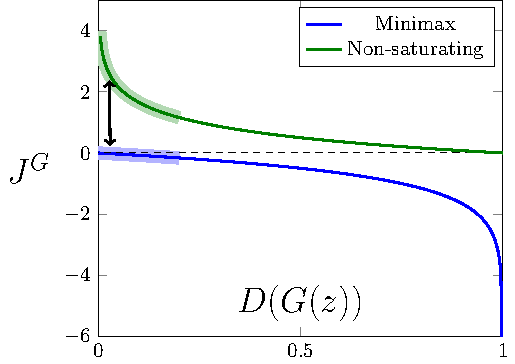
\includegraphics[width=0.8\textwidth, keepaspectratio]{images/loss_function}
\end{figure}
\end{frame}

\section{Models definition}

\begin{frame}
	\frametitle{GANs - Models definition}
	\begin{itemize}
		\item Different architectures for different data types.
		\begin{itemize}
			\only<1>{\item Tuple of numbers? \alert{Fully Connected Neural Networks}}
			\only<2>{\item Text or sequences?  \alert{Recurrent Neural Networks}}
			\only<3>{\item Images?  \alert{Convolutional Neural Networks}}
		\end{itemize}
	\end{itemize}

% figures
\only<1>{
		\begin{figure}
			\centering
			\includesvg[width=0.7\textwidth]{images/nn.svg}
		\end{figure}
}

\only<2>{
	\begin{figure}
		\centering
		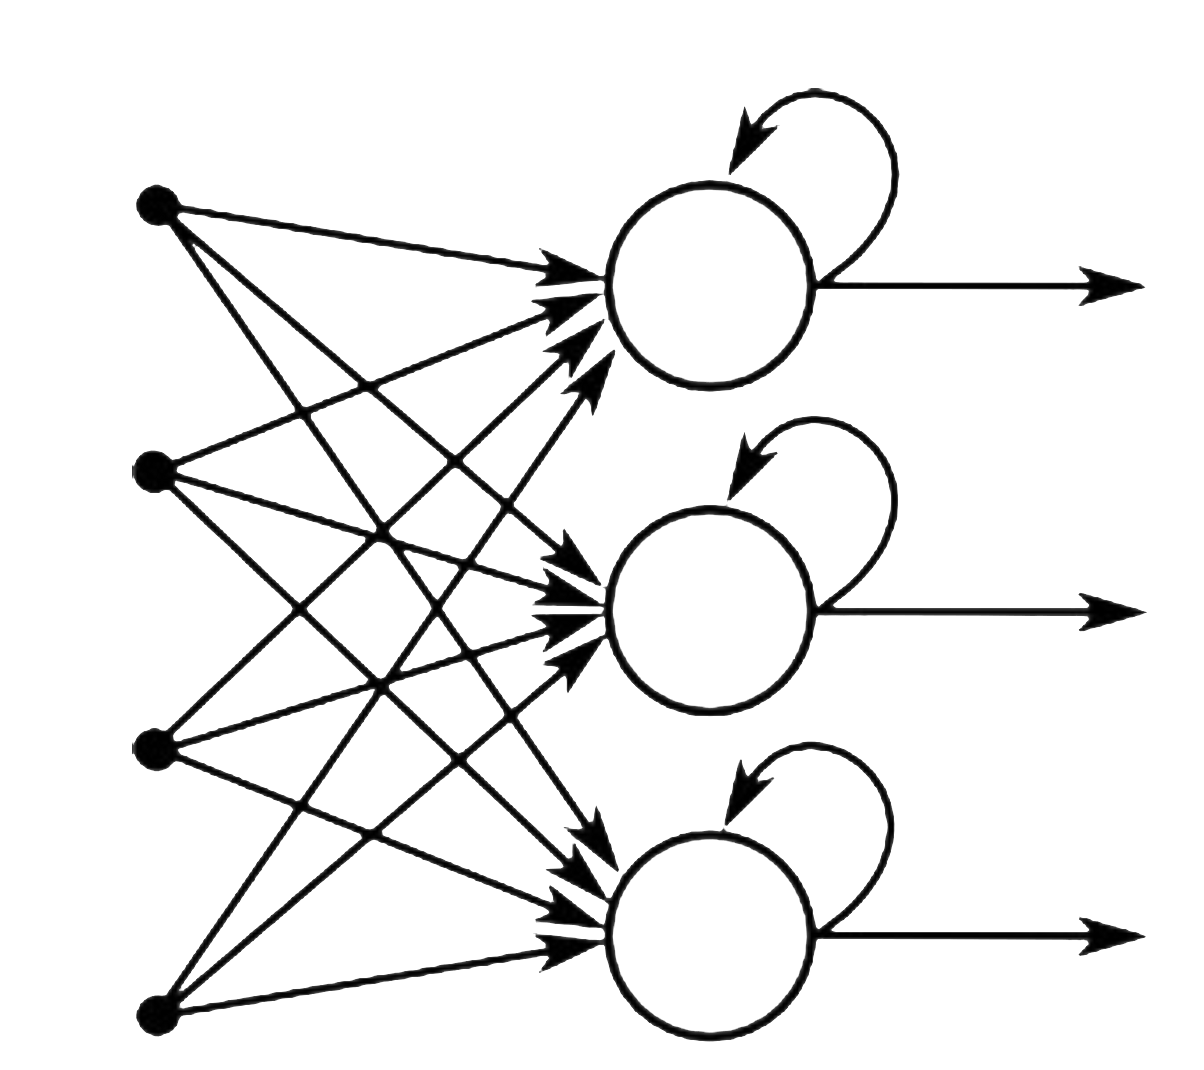
\includegraphics[width=0.6\textwidth]{images/recurrent.png}
	\end{figure}
}

\only<3>{
	\begin{figure}
		\centering
		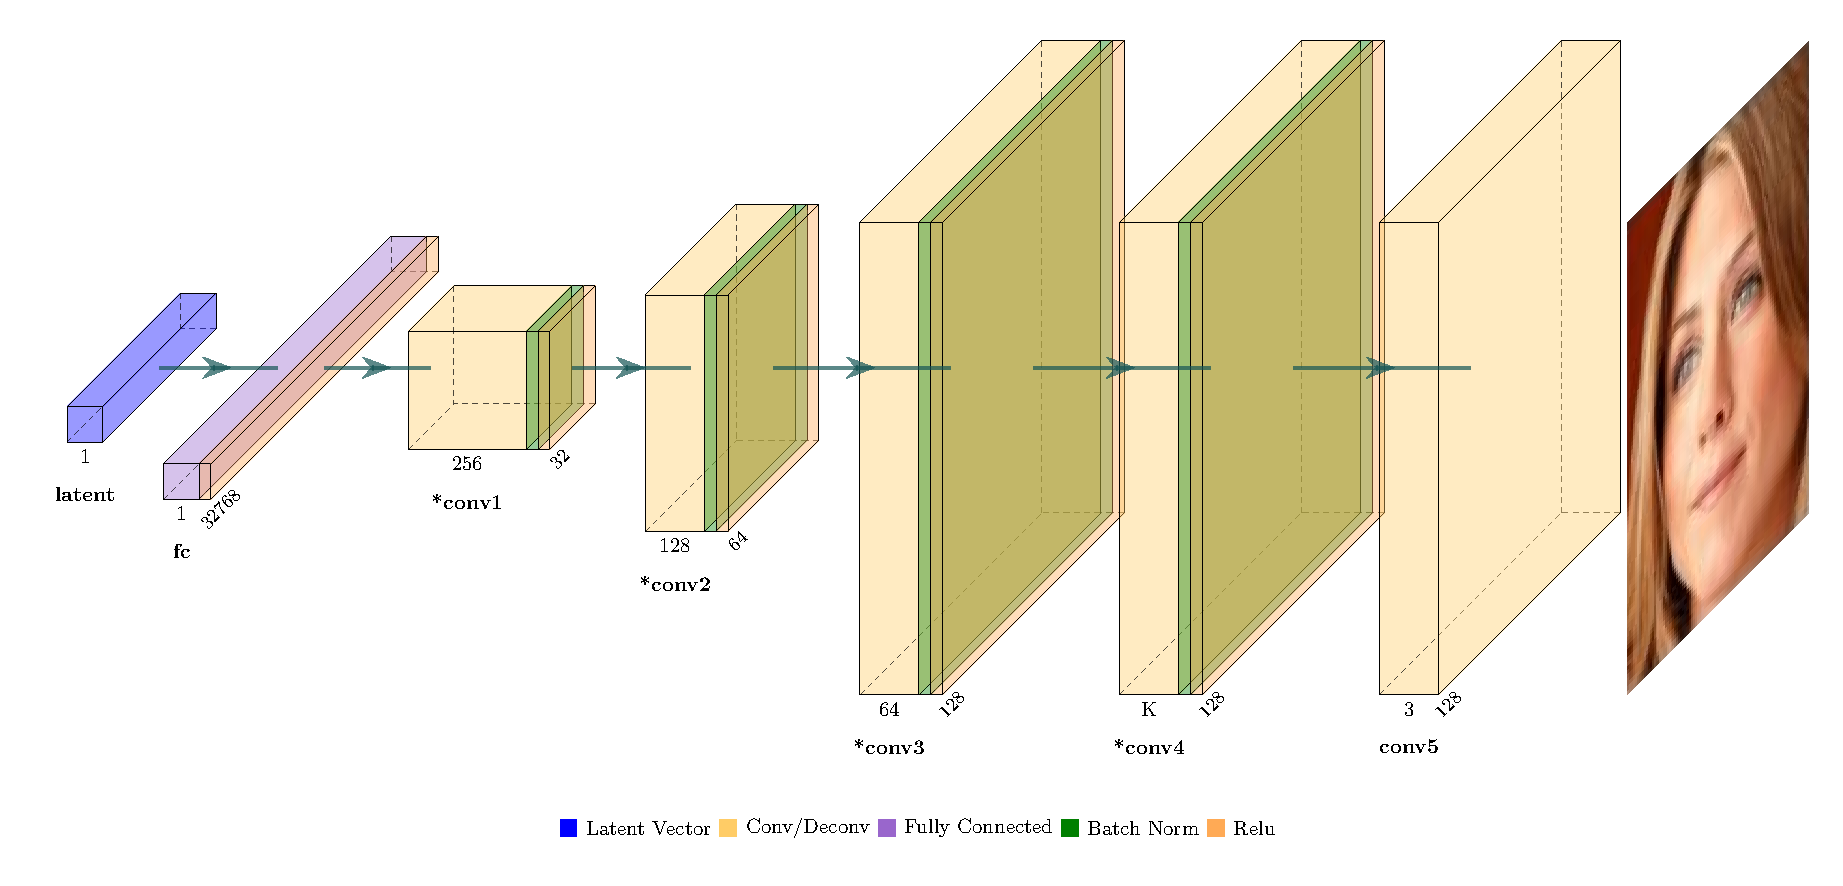
\includegraphics[width=1\textwidth]{images/cnn.pdf}
	\end{figure}
}
\end{frame}

\section{GANs Training}

\begin{frame}
	\frametitle{GANs - Training}
	\begin{itemize}
		\item D and G are \textbf{competing} against each other.
		\item \textbf{Alternating} execution of training steps.
		\item Use \textbf{minibatch stochastic gradient descent/ascent}.
	\end{itemize}
	\begin{figure}
		\centering
		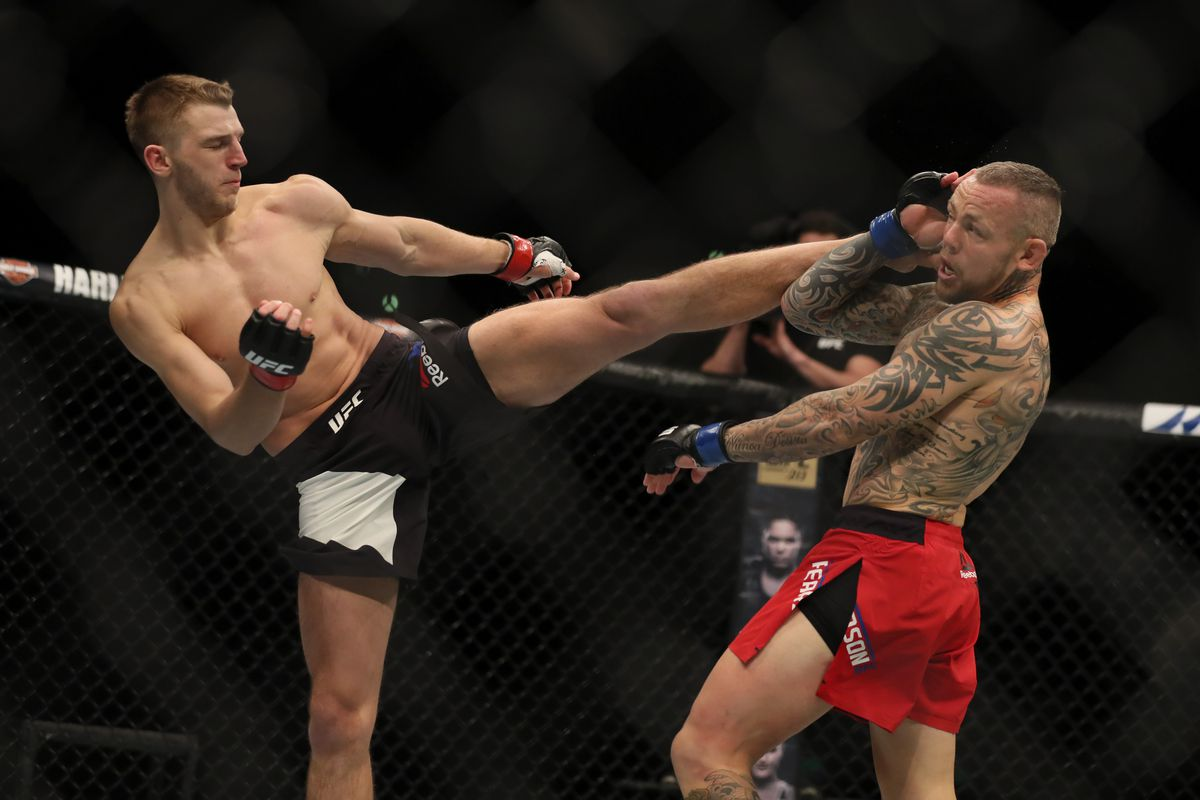
\includegraphics[width=0.7\textwidth]{images/fight.jpg}
	\end{figure}
\end{frame}

\begin{frame}
\setbeamercolor{normal text}{fg=gray,bg=}
\setbeamercolor{alerted text}{fg=black,bg=}
\usebeamercolor{normal text}
	\frametitle{GANs - Training - Discriminator}
	How to \textbf{train} the \textbf{discriminator}? \\
	Repeat from 1 to \textbf{k}:
		\begin{enumerate}
			\item<1-> \alert<+>{Sample minibatch of $m$ noise samples ${z^{(1)},\dots,z^{(m)}}$ from $p_z(z)$}
			\item<2-> \alert<+>{Sample minibatch of $m$ examples ${x^{(1)},\dots,x^{(m)}}$ from $p_{data}(x)$}
			\item<3-> \alert<+>{Update \textcolor{red}{\textbf{D}}:
		\begin{equation*}
			\mathbf{J} =  \underbrace{\frac{1}{m} \sum_{i=1}^{m} \log \textcolor{red}{\mathbf{D}}(x^{(i)}) + \log(1 - \textcolor{red}{\mathbf{D}}(\textcolor{real}{\mathbf{G}}(z^{(i)})))}_{\text{D performance}}
		\end{equation*}
	\LARGE		
	\begin{equation*}
	\theta_{\textcolor{red}{d}} = \theta_{\textcolor{red}{d}} + \lambda \nabla_{\theta_{\textcolor{red}{d}}} \mathbf{J}
	\end{equation*}	
}
		\end{enumerate}
\end{frame}

\begin{frame}
\setbeamercolor{normal text}{fg=gray,bg=}
\setbeamercolor{alerted text}{fg=black,bg=}
\usebeamercolor{normal text}
	\frametitle{GANs - Training - Generator}
	How to \textbf{train} the \textbf{generator}? \newline
	Update executed \textbf{only once} after \textcolor{red}{\textbf{D}} updates:
	\begin{enumerate}
		\item<1-> \alert<+>{Sample minibatch of $m$ noise samples ${z^{(1)},\dots,z^{(m)}}$ from $p_z(z)$}
		\item<2-> \alert<+>{Update \textbf{\textcolor{real}{G}}:
			\begin{equation*}
			\mathbf{J} = \underbrace{\frac{1}{m} \sum_{i=1}^{m} \log( \textcolor{red}{\mathbf{D}}(\textcolor{real}{\mathbf{G}}(z^{(i)})))}_{\text{G performance}}
			\end{equation*}
			\LARGE
			\begin{equation*}
			\theta_{\textcolor{real}{g}} = \theta_{\textcolor{real}{g}}  + \lambda \nabla_{\theta_{\textcolor{real}{g}}} \mathbf{J}
			\end{equation*}
}
	\end{enumerate}
\end{frame} 

\begin{frame}
	\frametitle{GANs - Training - Considerations}
	\begin{itemize}
		\item Optimizers: Adam, Momentum, RMSProp.
		\item \textbf{Arbitrary number} of steps or epochs.
		\item Training is completed when D is \textbf{completely fooled} by G.
		\item Goal: reach a \textbf{Nash Equilibrium} where the best D can do is random guessing.
	\end{itemize}
 \end{frame}
 
\section{Types of GANs}

\begin{frame}
	\frametitle{Types of GANs}
	Two big families:
	\begin{itemize}
		\item \textbf{Unconditional} GANs (just described).
		\item \textbf{Conditional} GANs \citep{mirzaConditionalGenerativeAdversarial2014}.
	\end{itemize}
\end{frame}

\begin{frame}
	\frametitle{Conditional GANs}
	\begin{itemize}
		\item \textbf{Both} $G$ and $D$ are \textbf{conditioned} on some extra information $ \color{red} \mathbf{y}$.
		\item In \textbf{practice}:  perform conditioning by feeding $\color{red} \mathbf{y}$ into the discriminator and generator.
	\end{itemize}
	\vspace{-1cm}
	\begin{figure}
		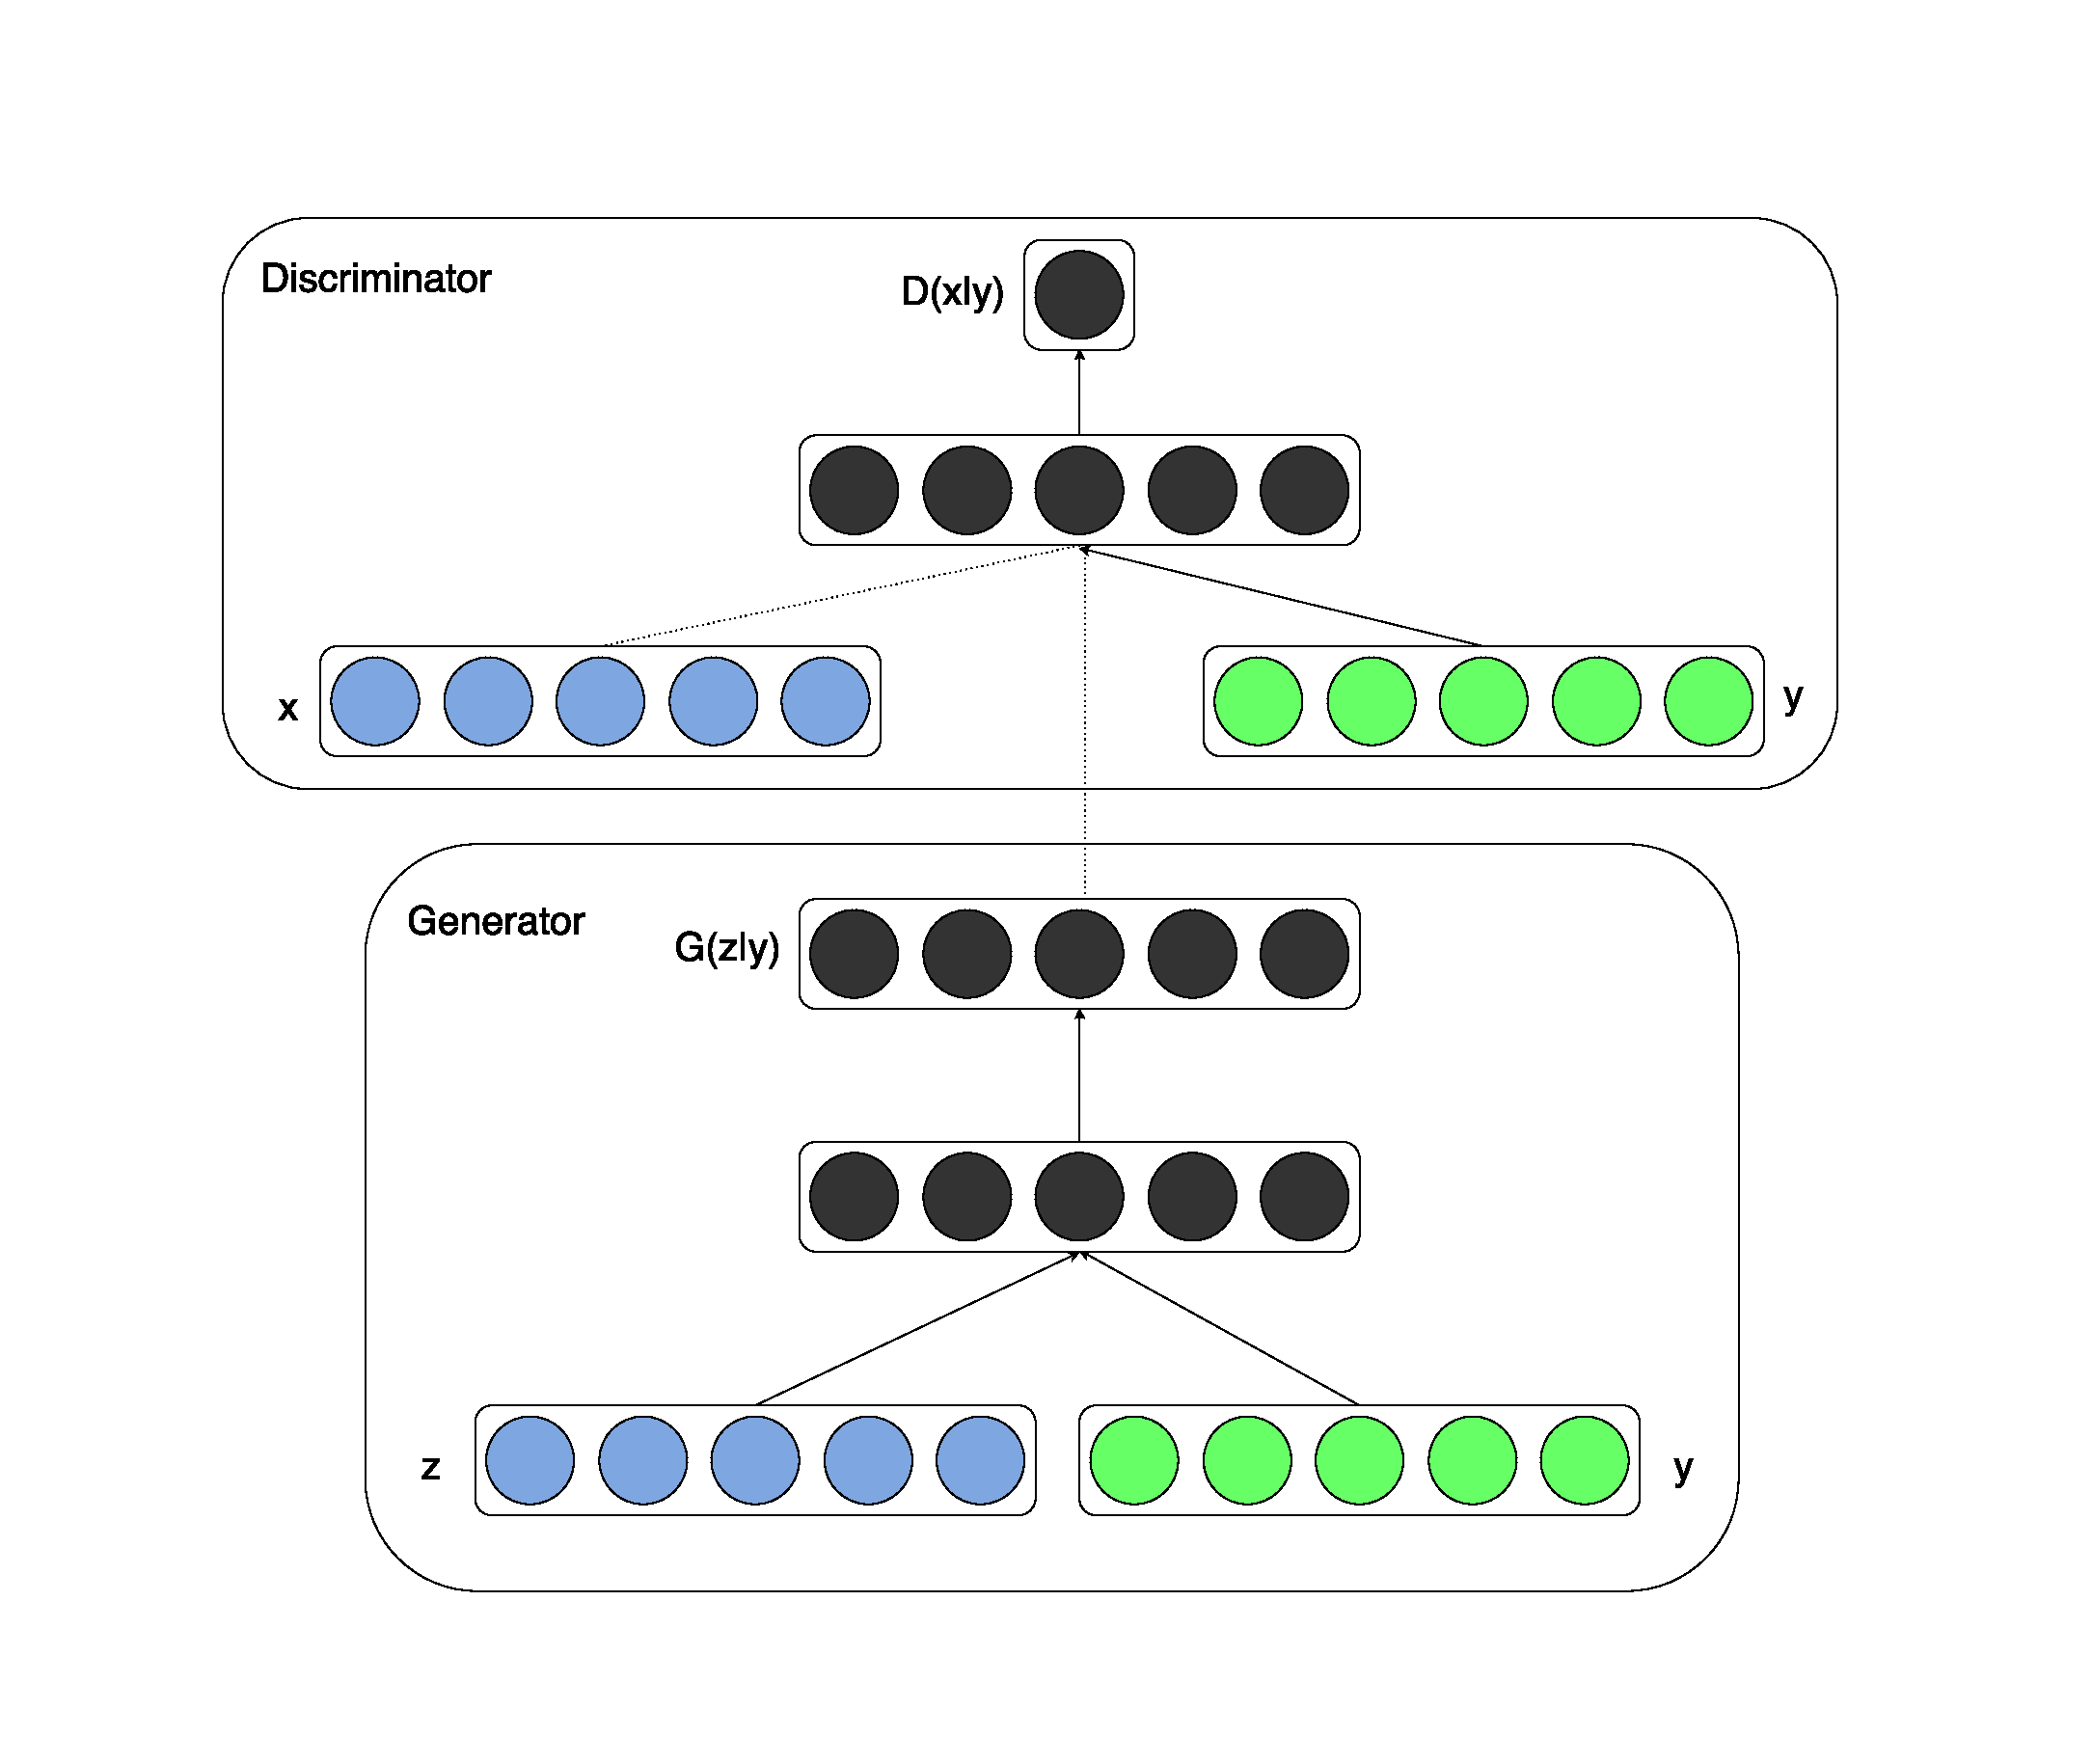
\includegraphics[height=0.8\textheight]{images/diagram.pdf}
		\vspace{-1cm}
		\caption{From \cite{mirzaConditionalGenerativeAdversarial2014}}
	\end{figure}
\end{frame}

\begin{frame}
	\frametitle{Conditional GANs}
	The GANs game becomes:
	$$ 
	\min_G \max_D \underset{x \sim p_{data}(x| \textcolor{red}{\mathbf{y}})}{\mathbb{E}} [\log D(x, \textcolor{red}{\mathbf{y}})]  +\underset{z \sim p_z(z)}{\mathbb{E}}[\log(1 - D(G(z|\textcolor{red}{\mathbf{y}}),\textcolor{red}{\mathbf{y}}))]
	$$

	\setbeamercolor{block body}{bg=red!30!white}
	\begin{block}{}
		Notice: the same representation of the condition has to be presented to both network.
	\end{block}
\end{frame}

\section{GANs Applications}

{
\usebackgroundtemplate{
	\vbox to \paperheight{\vfil\hbox to \paperwidth{\hfil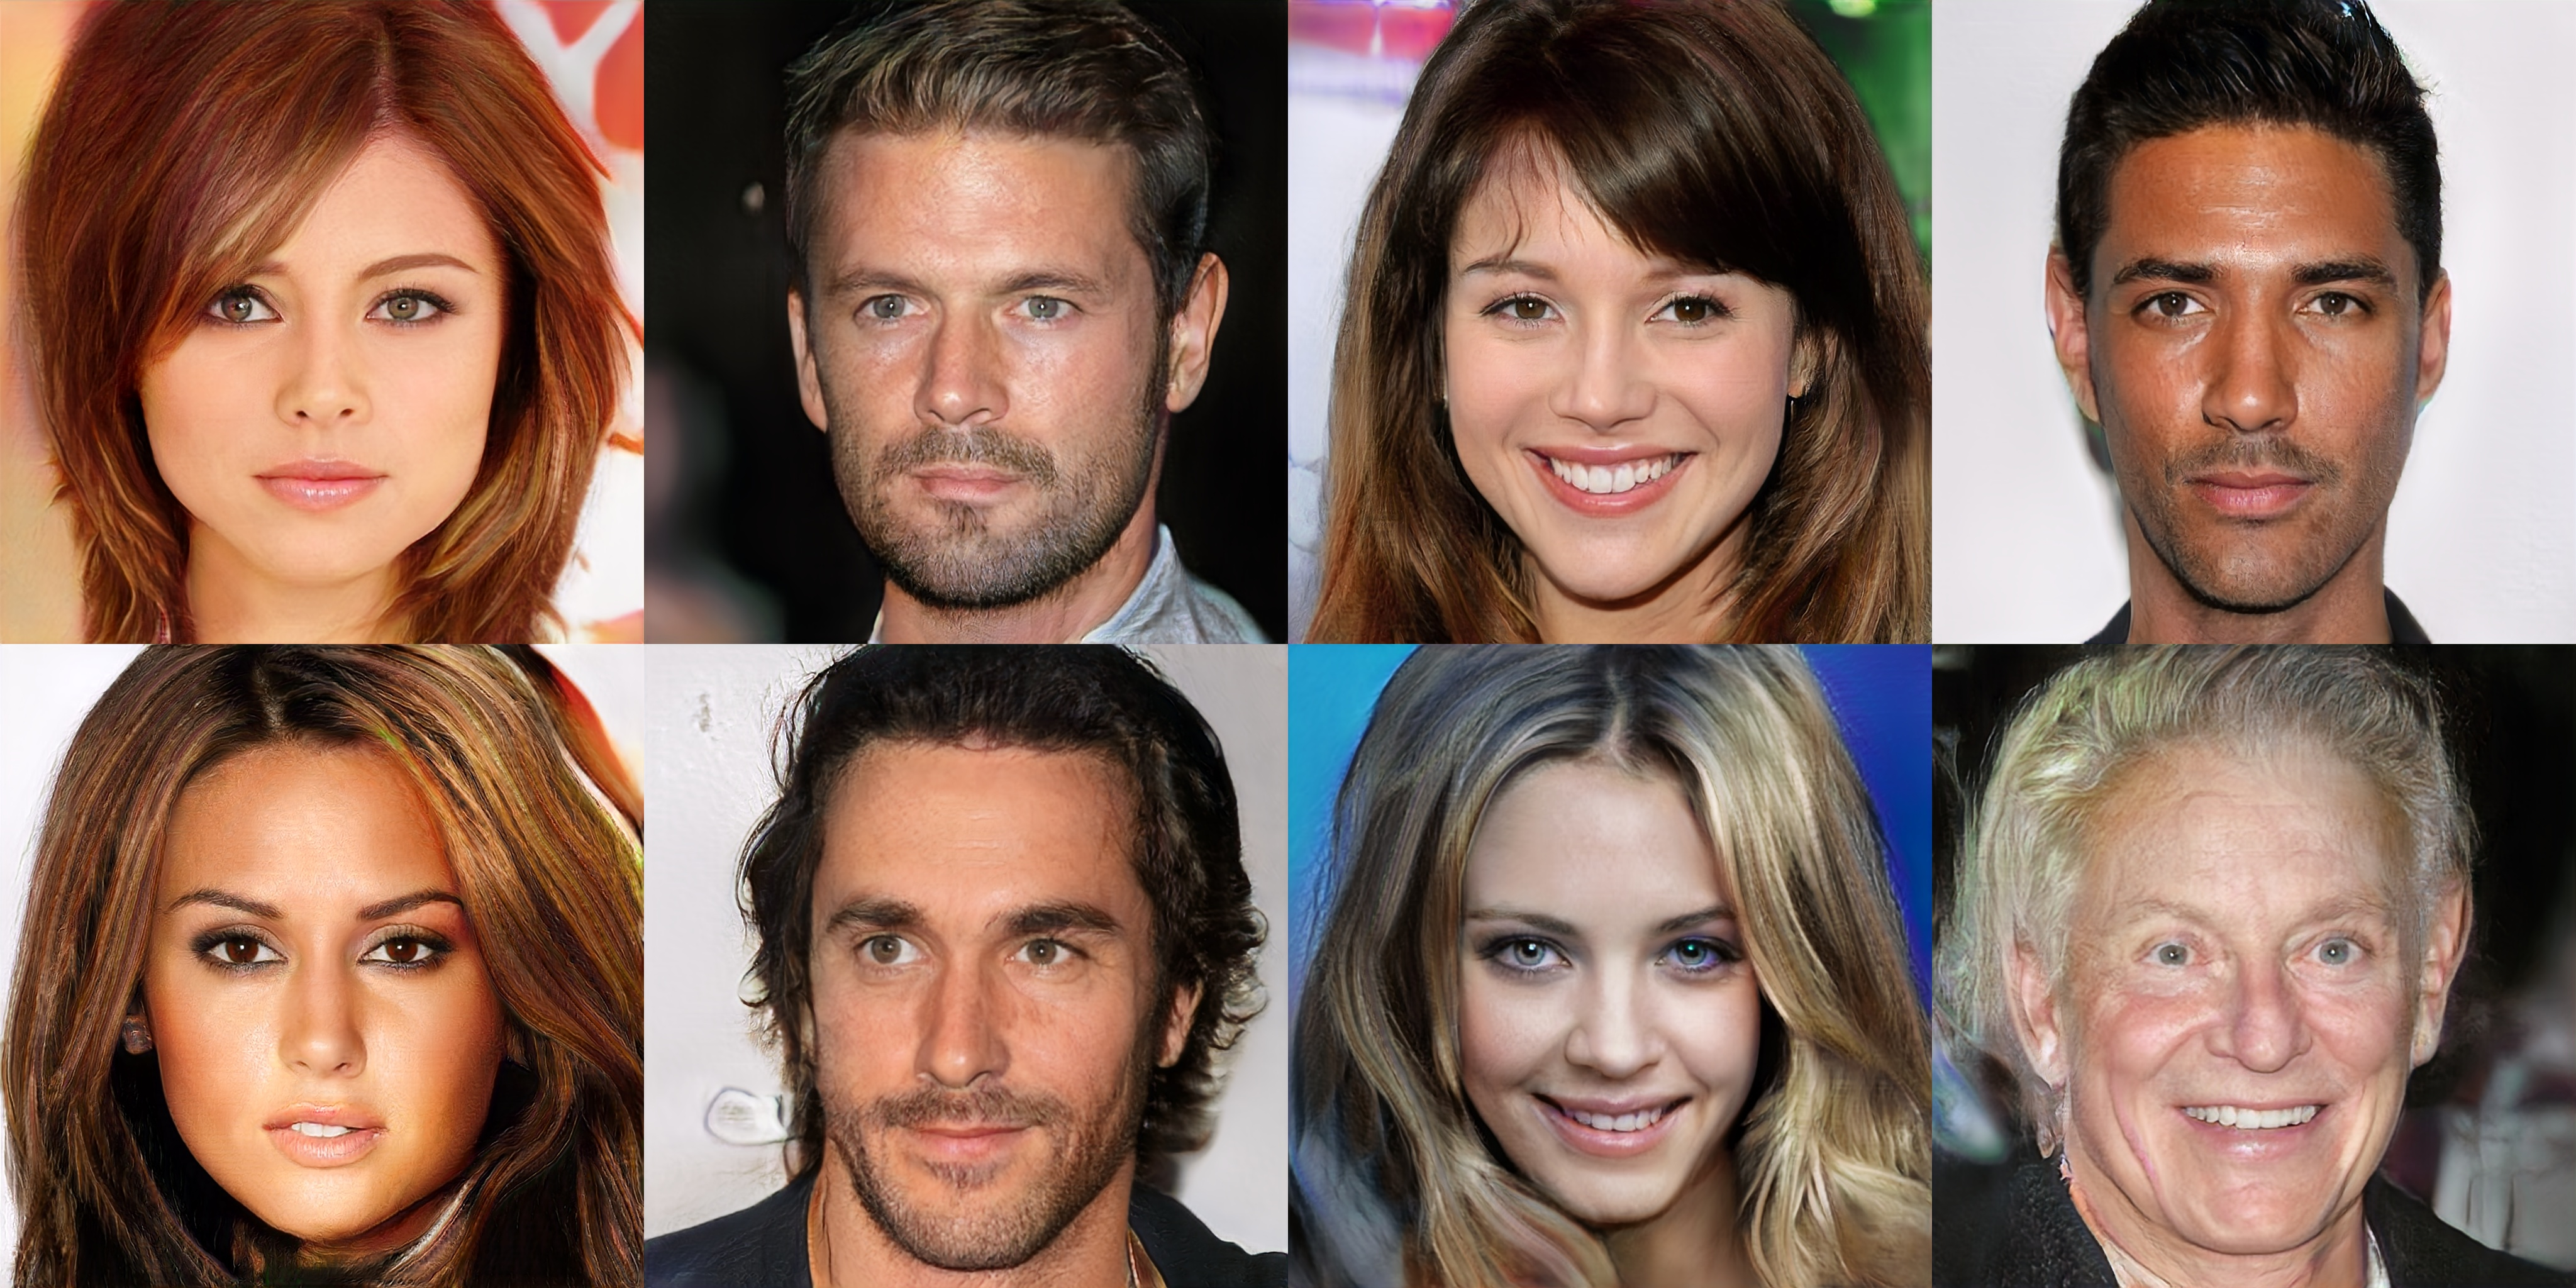
\includegraphics[width=\paperwidth]{images/celeb1024-results}\hfil}\vfil}
}
	\begin{frame}
		\frametitle{Unconditional - Face Generation - \cite{karrasProgressiveGrowingGANs2017}}
	\end{frame}
}

{
\usebackgroundtemplate{
	\vbox to \paperheight{\vfil\hbox to \paperwidth{\hfil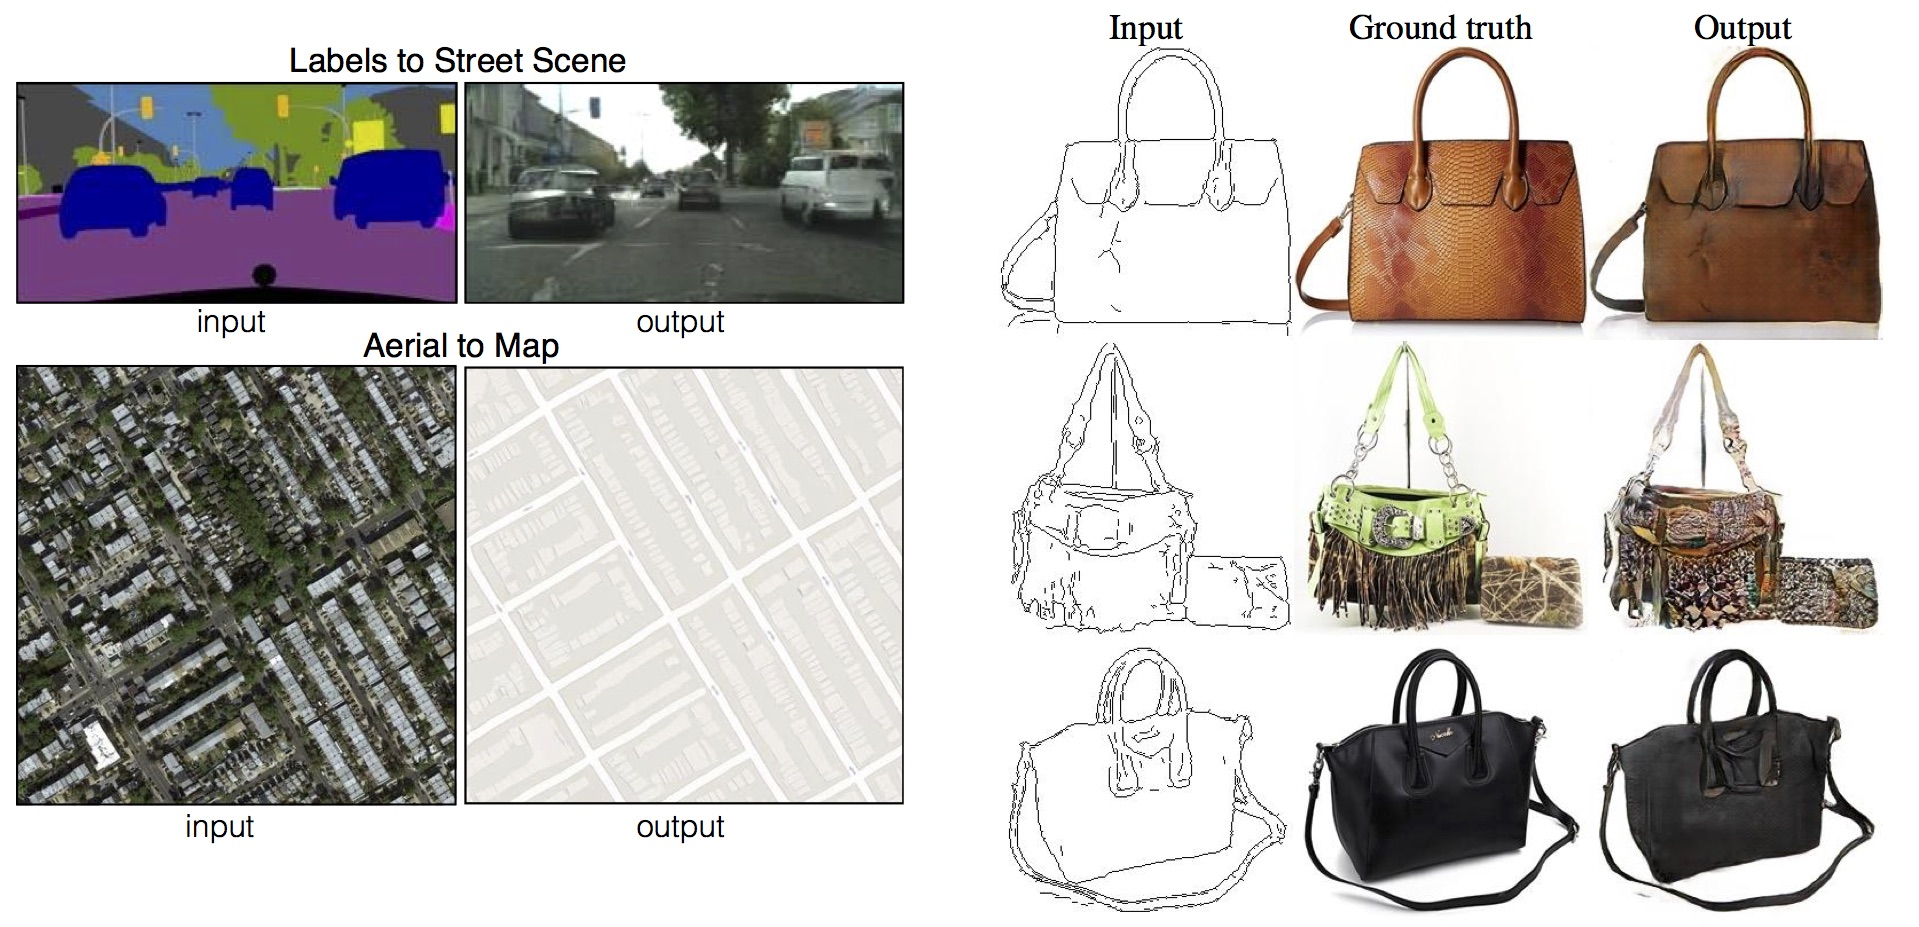
\includegraphics[width=\paperwidth]{images/im2im}\hfil}\vfil}
}
	\begin{frame}
		\frametitle{Conditional - Domain Translation - \cite{isolaImagetoImageTranslationConditional2016a}}
	\end{frame}
}


	\begin{frame}
		\frametitle{Conditional - Semantic Image Synthesis - \cite{parkSemanticImageSynthesis2019}}
		\animategraphics[loop,autoplay,width=1\textwidth]{0.5}{images/spade/}{0}{17}
	\end{frame}


{
\usebackgroundtemplate{
	\vbox to \paperheight{\vfil\hbox to \paperwidth{\hfil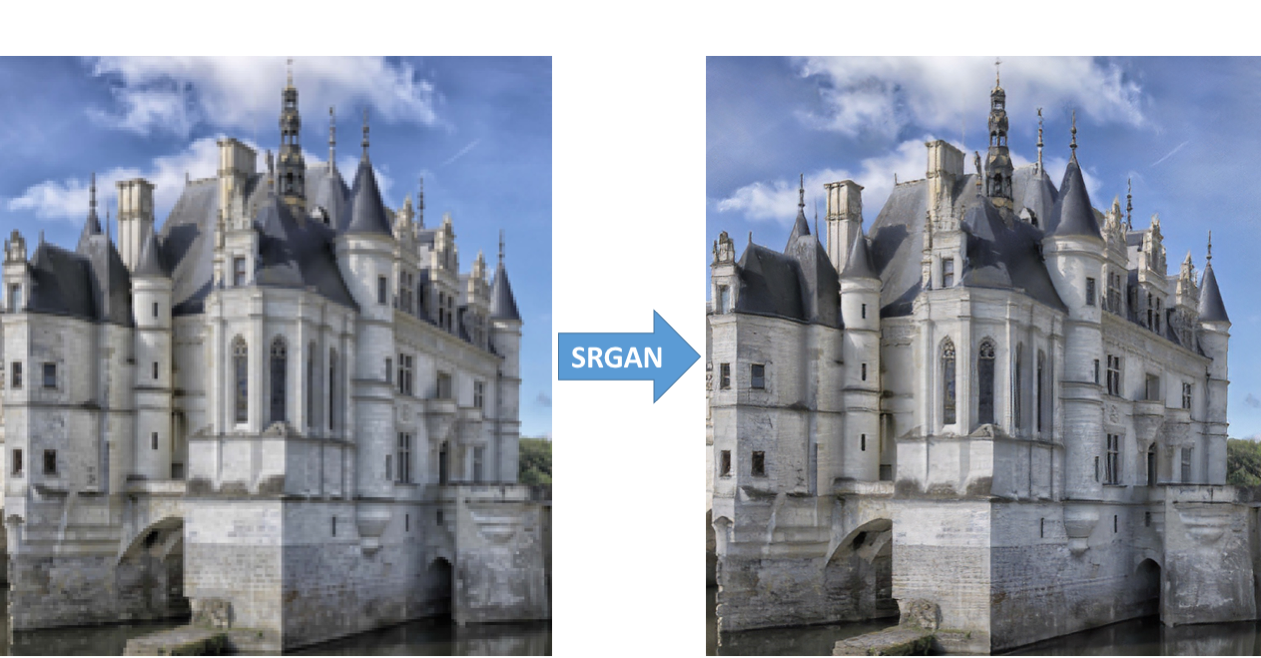
\includegraphics[width=\paperwidth, keepaspectratio]{images/SRGAN.png}\hfil}\vfil}
}
	\begin{frame}
		\frametitle{Conditional - Image Super Resolution - \cite{ledigPhotoRealisticSingleImage2016}}
	\end{frame}
}

% \begin{frame}[standout]
%	\begin{center}
%	\Large	Thank you for your attention! \hfill \\
%	\Large	Questions?
% 	\end{center}
%\end{frame}

\appendix

\begin{frame}{Real-world GANs }
	\begin{itemize}
		\item Semi-Supervised Learning \citep{salimansImprovedTechniquesTraining2016a}
		\item Image Generation (almost all GAN papers)
		\item Image Captioning
		\item Anomalies Detection \citep{zenatiEfficientGANBasedAnomaly2018a}
		\item Program Synthesis \citep{ganinSynthesizingProgramsImages2018}
		\item Genomics and Proteomics \citep{killoranGeneratingDesigningDNA2017} \citep{decaoMolGANImplicitGenerative2018}
		\item Personalized GANufactoring \citep{hwangLearningHumanExpertise2018}
		\item Planning
	\end{itemize}
\end{frame}

%% reference
\begin{frame}[allowframebreaks]
	 \bibliographystyle{mydinat}
	\bibliography{bibl.bib}
\end{frame}

\end{document}